\chapter{Model}



Nun da man mit dem Begriff MNIST vertraut sein sollte und auch weiss, wie man die Daten in ein eigenes Python Programm einbinden kann, kann mit dem nächsten Schritt, dem Model, fortgefahren werden. 
Um den Begriff des Models möglichst knapp zusammenzufassen, eignet sich der Begriff des Systems. Das Model bildet dabei ein System, welches einen Input entgegennimmt, mit diesem Berechnungen durchführt und schlussendlich einen entsprechenden Output liefert. Die wichtigsten Bausteine im Model sind dabei die künstlichen Neuronen, die Gewichte, welche diese verbinden und der Bias, welcher als externer Input dient. Je nach Anordnung und Aufbau dieser Elemente kann zwischen etlichen verschiedenen Models unterschieden werden. Für diesen Workshop wird ein Model namens Softmax Regression verwendet. Um dieses allerdings möglichst einfach zu beschreiben, macht es Sinn, erstmals die Logistic Regression zu erläutern.


\section{Logistic Regression}
Wie die Grafik \ref{fig:logistic_regression} zeigt, wird der Input bei der Logistic Regression durch die Gewichte propagiert und schlussendlich die Summe der einzelnen Neuronen gebildet. Dieser Wert wiederum wird in die Aktivierungsfunktion weitergegeben, welche zwischen zwei möglichen Ausgangswerten entscheidet. Dies macht beispielsweise Sinn, wenn man sich zum Ziel setzt mit Hilfe eines neuronalen Netzes festzustellen, ob es sich bei einem gewissen Input um ein Element eines gewissen Typs handelt oder nicht. Es wird also zwischen Ja und Nein unterschieden.
\begin{figure}[!ht]
\centering
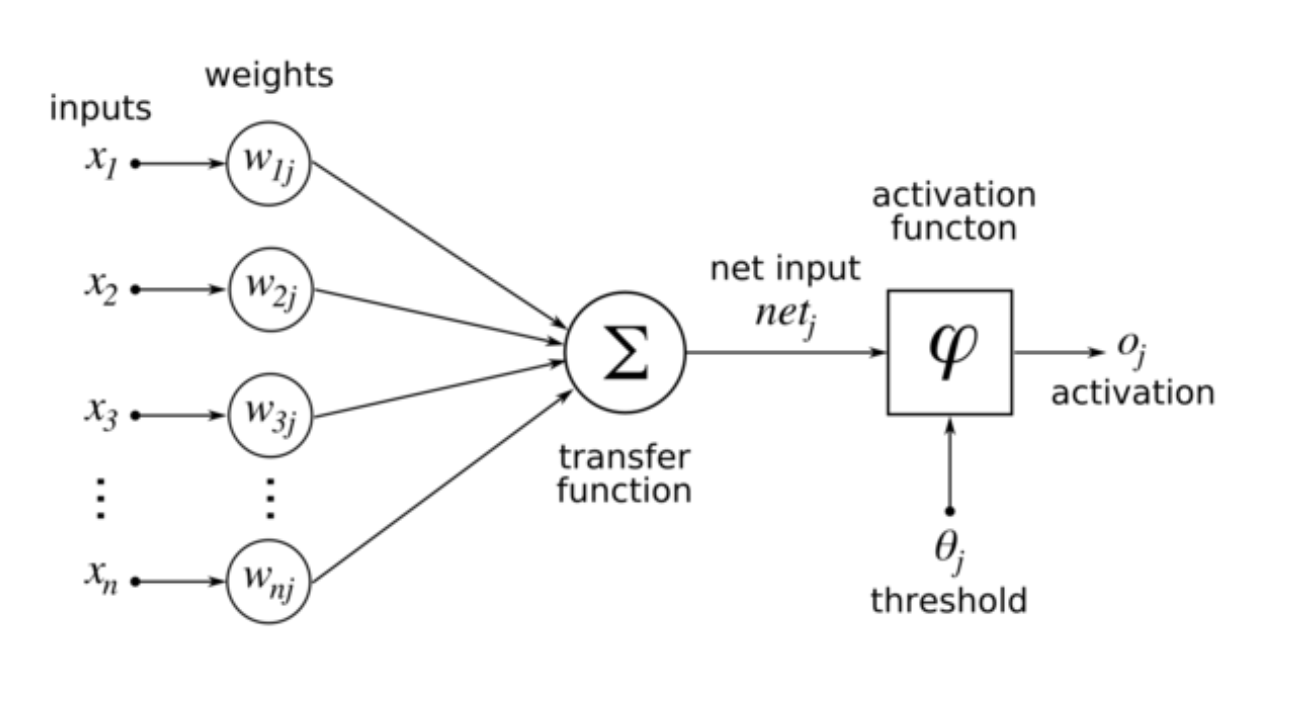
\includegraphics[width=1.00\textwidth]{images/logistic}
\caption{Logistic Regression}
\label{fig:logistic_regression}
\end{figure}

\section{Softmax Regression}
Wie aus der Grafik \ref{fig:softmax_regression} zu entnehmen ist, verfügt die Softmax Regression prinzipiell über einen sehr ähnlichen Aufbau wie die Logistic Regression. Der wesentliche Unterschied zur Logistic Regression liegt jedoch im Output des Models. Im Gegensatz zur Logistic Regression werden die Ausgänge der einzelnen Neuronen nicht in einer Summe an eine Aktivierungsfunktion weitergeleitet, es gibt N Summen der Neuronen, welche in die Softmax Funktionseinheit propagiert werden. Diese entscheidet nun nicht einfach zwischen Ja und Nein, sondern gibt eine Wahrscheinlichkeit für jeden der N möglichen Ausgänge ab, dass es sich um diesen handelt. Dieses Muster eignet sich besonders gut für die Problemstellung der Ziffernerkennung. Sie liefert jeweils für jede Ziffer zwischen 0 und 9 einen Wahrscheinlichkeitswert, der angibt, wie wahrscheinlich es für das Model ist, dass der Input, in diesem Fall ein Bild, eine 0,1,2,…, 9 zeigt. Sucht man jetzt den höchsten Wahrscheinlichkeitswert aus diesem Vektor, erhält man jene Ziffer, von der das Model glaubt, sie auf dem Bild erkannt zu haben.
\begin{figure}[!ht]
\centering
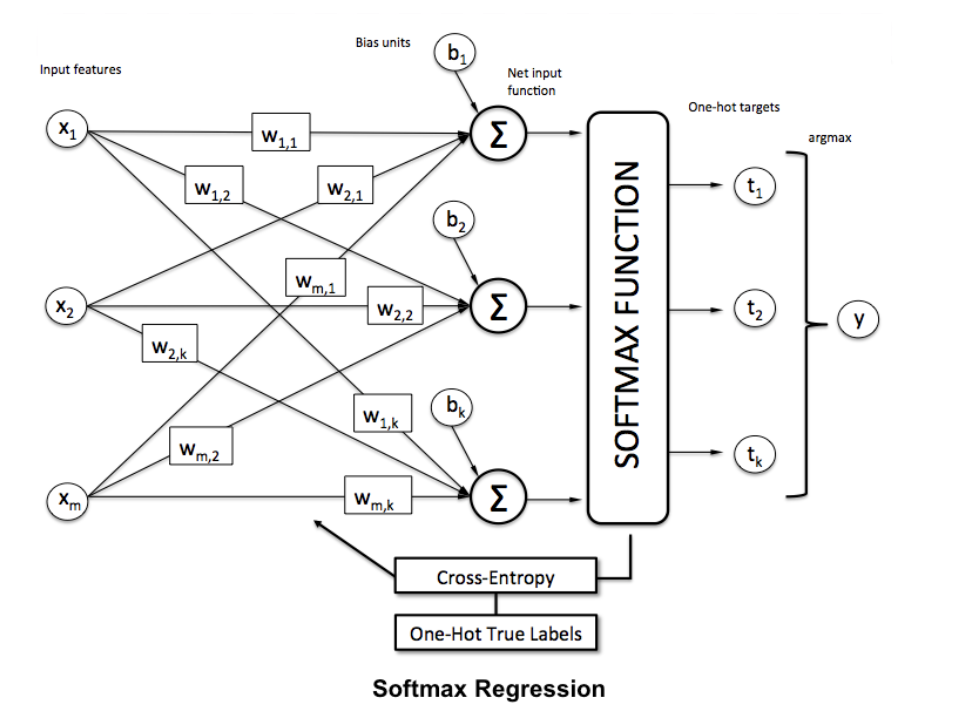
\includegraphics[width=1.00\textwidth]{images/softmax}
\caption{Softmax Regression}
\label{fig:softmax_regression}
\end{figure}

\section{Implementierung}

Um das Model im Python Skript zu implementieren, müssen zuerst einmal die benötigten TensorFlow Variablen und Placeholder angelegt werden.
Der erste Placeholder der gebraucht wird, ist jener der Input-Images. Jedes Bild der MNIST Daten besteht aus 28x28 Pixeln. Reiht man diese Pixel hintereinander, erhält man einen Zeilenvektor der Länge 784. Da die Bilddaten auf diese Weise gespeichert werden sollen, wird mit folgender Zeile ein passender Placeholder angelegt.

\lstset{language=Python}
\definecolor{listinggray}{gray}{0.95} 
\definecolor{keyword}{rgb}{0.4, 0, 0.1} 
\definecolor{comment}{rgb}{0, 0.4, 0}
% Zuweisen der Farben zu den entsprechenden Elementen ... 
\lstset{keywordstyle=\color{keyword}\bfseries} 
\lstset{commentstyle=\color{comment}} 
\lstset{backgroundcolor=\color{listinggray}}

\begin{lstlisting}
x = tf.placeholder(tf.float32, [None, 784], name='InputData')
\end{lstlisting}



Dieser kann eine beliebige Anzahl (None) an Bilddaten (1x784) im Format Float (Grauwerte zwischen 0 und 1) beinhalten und trägt den Namen InputData. Als nächstes wird ein Placeholder gebraucht, der zu jedem Bild das dazugehörige Label abspeichert. Da wir die Labels als One-Hot Vektor geladen haben und 10 mögliche Ausgänge existieren, bildet jedes Label einen Zeilenvektor der Länge 10 ab. Um so einen Placeholder anzulegen, wird folgender Befehl verwendet.

\lstset{language=Python}
\definecolor{listinggray}{gray}{0.95} 
\definecolor{keyword}{rgb}{0.4, 0, 0.1} 
\definecolor{comment}{rgb}{0, 0.4, 0}
% Zuweisen der Farben zu den entsprechenden Elementen ... 
\lstset{keywordstyle=\color{keyword}\bfseries} 
\lstset{commentstyle=\color{comment}} 
\lstset{backgroundcolor=\color{listinggray}}

\begin{lstlisting}
y = tf.placeholder(tf.float32, [None, 10], name = 'LabelData')
\end{lstlisting}

Analog zum InputData Placeholder kann auch dieser eine beliebige Anzahl (None) an Labels (1x10) im Format Float (Wahrscheinlichkeitswert zwischen 0 und 1) beinhalten und trägt den Namen LabelData.
Nachdem nun die Placeholder für den Input angelegt wurden, kann mit den nötigen, modellspezifischen Variablen fortgefahren werden. 
Der Befehl: 


\lstset{language=Python}
\definecolor{listinggray}{gray}{0.95} 
\definecolor{keyword}{rgb}{0.4, 0, 0.1} 
\definecolor{comment}{rgb}{0, 0.4, 0}
% Zuweisen der Farben zu den entsprechenden Elementen ... 
\lstset{keywordstyle=\color{keyword}\bfseries} 
\lstset{commentstyle=\color{comment}} 
\lstset{backgroundcolor=\color{listinggray}}

\begin{lstlisting}
W = tf.Variable(tf.zeros([784, 10]), name='Weights')
\end{lstlisting}

erzeugt eine Variable, welche alle Gewichte zwischen Input und Output beinhaltet. Dies ergibt bei 784 Eingängen und 10 Ausgängen 7840 Gewichte insgesamt. Die letzte benötigte Variable ist jene der Bias-Werte. Für jeden der möglichen Ausgänge wird jeweils ein Wert benötigt, was zu einem Zeilenvektor der Länge 10 führt. Dieser wird folgendermaßen implementiert.


\lstset{language=Python}
\definecolor{listinggray}{gray}{0.95} 
\definecolor{keyword}{rgb}{0.4, 0, 0.1} 
\definecolor{comment}{rgb}{0, 0.4, 0}
% Zuweisen der Farben zu den entsprechenden Elementen ... 
\lstset{keywordstyle=\color{keyword}\bfseries} 
\lstset{commentstyle=\color{comment}} 
\lstset{backgroundcolor=\color{listinggray}}

\begin{lstlisting}
b = tf.Variable(tf.zeros([10]), name = 'Bias')
\end{lstlisting}



Das letzte Stück Code welches benötigt wird, ist jenes des Models an sich.


\lstset{language=Python}
\definecolor{listinggray}{gray}{0.95} 
\definecolor{keyword}{rgb}{0.4, 0, 0.1} 
\definecolor{comment}{rgb}{0, 0.4, 0}
% Zuweisen der Farben zu den entsprechenden Elementen ... 
\lstset{keywordstyle=\color{keyword}\bfseries} 
\lstset{commentstyle=\color{comment}} 
\lstset{backgroundcolor=\color{listinggray}}    
   
\begin{lstlisting}
with tf.name_scope('Model'):
    pred = tf.nn.softmax(tf.matmul(x,W) + b)
\end{lstlisting}
    
    
Die erste Zeile hat prinzipiell keine funktionalen Auswirkungen auf das Model, jedoch hilft es TensorBoard dabei den Graphen übersichtlicher darzustellen, wie man später bemerken wird.
Die zweite Zeile erzeugt nun das eigentliche Model, welches auf Basis der zuvor angelegten Placeholder und Variablen eine Softmax entsprechende Schätzung liefert, um welche Ziffer es sich handelt.





\label{cha:Model}
